\subsection{Spatial Memory Streaming Prefetcher}
\label{sec:smsPrefetcher}

The Spatial Memory Streaming (SMS) Prefetcher is a spatial locality
prefetcher which ideas was first presented in \cite{SMS}, it tries to
exloit the relationship between a memory page, and a cache line.

Since a memory page is larger than a cache line, the memory page is
fragmented across several cache lines, and even though the page is in
memory, only parts of it may be in the cache.  When designing
operating systems and database management systems, the system designer
will optimize the design for the memory page size in order to limit
the amount of bandwidth and access to the disk. In order to achieve
this, large and complex data structures will have to be chunked up into
smaller and equal structures that fit into a single memory page.

When performing large scale operations on these data structures, for
example a database search, the program might sit in a loop while it
processes several of these page sized data structures. For instance,
while processing these pages the program might always access a page
header, a B-tree key-pointer and a pointer collection at the end of
the page. By recording the access pattern on a single page the pattern may
be used on multiple pages each time the program accesses a new page
with the same program counter and the same page offset.

\begin{figure}[H]
  \centering
  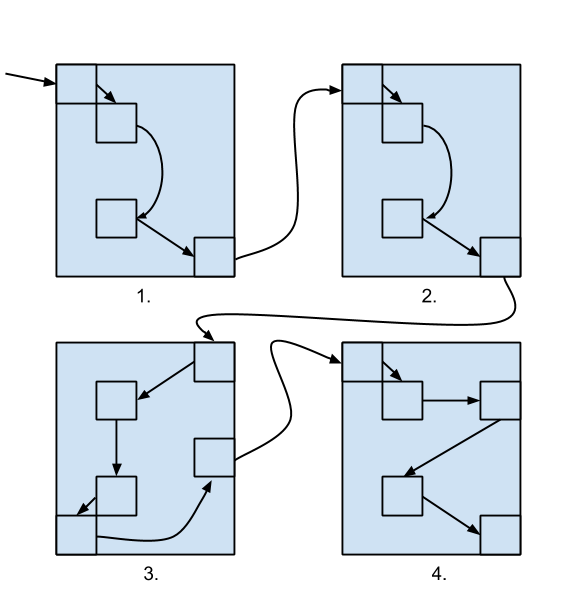
\includegraphics[scale=0.35]{./figures/sms_pattern.png}
  \caption{Cache blocks accessed across memory pages}
  \label{fig:sms_pattern}
\end{figure}

Figure \ref{fig:sms_pattern} shows the opportunities that SMS tries to exploit, here pages 1 and 2 have exactly the same access pattern. Page 4 has a similar entry point but differs from 1 and 2 in that it has one more cache block. Altought Page 3 has some similar blocks it differs in entry. SMS will exploit the pattern that was recorded on page 1 to prefetch the blocks in Page 2 and 4.

\subsubsection{How it works}
SMS uses two different tables in its implementation. The Active
Generation Table (AGT) which is used when recording spatial pattern,
and the Page History Table (PHT) which stores recorded patterns. 

A generation is the time over which SMS records access to a spatial
memory region. The spatial memory region is the collection of cache
lines the SMS considers as a larger memory structure and it emulates
the operating system memory page. The memory access that triggers a
generation is referred to as a trigger access and it is the first
access to memory region which is not currently being recorded in the
AGT. The generation ends when one of the accessed cache lines that
have been accessed during the generation is invalidated or evicted
from the cache.  When a generation ends it is transferred from the AGT
to the PHT if it has two or more accesses within the spatial
region. In order to make the implementation easier the AGT is divided
into two tables, the filter table and the accumulation table.  Upon a
trigger access the generation is first inserted into the filter table,
when the spatial region is accessed a second time, it is moved from
the filter table to the accumulation table. All subsequent accesses
updates the spatial pattern in the accumulation table.  An entry in
the AGT consist of a tag, which is the base address of the spatial
region, the program counter and the offset that triggered the
generation and a spatial bit pattern of the cache lines which has been
accessed during the generation. 

\begin{table}[htbp]
  \centering
  \begin{tabular}{| c | c |}
    \hline
    {\bf Access} & {\bf Action} \\ \hline
    A + 0 & Generation A [0001]\\ \hline
    A + 1 & Generation A [0011]\\ \hline
    A + 3 & Generation A [1011]\\ \hline
    B + 2 & Generation B [0100]\\ \hline
    C + 1 & Generation C [0010] \\ \hline
    evict A + 1 & Move Generation A to PHT\\ \hline
    A + 0 & Generation A' [0001]\\ \hline
    A + 2 & Generation A' [0101]\\ \hline
    B + 3 & Generation B [1100] \\ \hline
    invalidate B + 2 & Move Generation B to PHT\\ \hline
    evict C + 1 & Remove Generation C from AGT \\ \hline    
  \end{tabular}
  \caption{The lifetime of Generations}
  \label{tab:generation}
\end{table}
Table \ref{tab:generation} shows an access sequence and the
actions applied to the generations and their pattern in the AGT.

Upon a trigger access SMS searches the history table for a pattern
that can be used to predict which addresses will be accessed.  A PHT
entry has a tag which is the program counter and the spatial region
offset of the trigger access to the recorded generation, and the
recorded spatial pattern that was recorded during the generation.
When searching through the PHT the current program counter and spatial
region offset is compared to the PHT tag. If there is a match in the
PHT a set of predicted addresses is constructed from the spatial
region base address and the set of block offsets recorded in the
spatial pattern. These addresses is then put into a queue of memory
addresses to be streamed into the cache.
 

{\bf (references, citations)}
